\documentclass[11pt, oneside]{article}   	% use "amsart" instead of "article" for AMSLaTeX format
\usepackage{geometry}                		% See geometry.pdf to learn the layout options. There are lots.
\geometry{letterpaper}                   		% ... or a4paper or a5paper or ... 
%\geometry{landscape}                		% Activate for rotated page geometry
%\usepackage[parfill]{parskip}    		% Activate to begin paragraphs with an empty line rather than an indent
\usepackage{graphicx}				% Use pdf, png, jpg, or eps§ with pdflatex; use eps in DVI mode
								% TeX will automatically convert eps --> pdf in pdflatex		
\usepackage{amssymb}
\usepackage{tabularx}				% To automatically wrap long column contents
\usepackage[dvipsnames]{xcolor}					% For page color
\pagecolor{white}					% For white page color

\usepackage{fancyhdr}

\pagestyle{fancy}
\fancyhf{}
%\fancyhead[LE,RO]{Rahul S.}
% \fancyhead[RE,LO]{Take Home Test}
%\fancyfoot[CE,CO]{\leftmark}
\fancyfoot[LE,CO]{\thepage}

\renewcommand{\headrulewidth}{2pt}
\renewcommand{\footrulewidth}{1pt}

\usepackage{hyperref}				% To insert URL
\hypersetup{						% hyperlink formatting
    colorlinks=true,
    linkcolor=blue,
    filecolor=magenta,      
    urlcolor=cyan,
    pdftitle={Sharelatex Example},
    bookmarks=true,
    pdfpagemode=FullScreen,
}

\title{\textbf{Take Home Test - Treau}}
\author{Rahul Subramanian}
%\date{}							% Activate to display a given date or no date

\begin{document}
\maketitle

\newpage
\section{Question}
1. Assess yourself, from 1 to 4, in the following areas or skills. We are not looking for a candidate to have experience with all, or even a majority, of these areas. This question is much less about the magnitude of the numbers and more about their relation – where do you think your strengths are?
\newline
\newline
1 = Very little or no experience
\newline
2 = Some experience, but not yet at a level of full competence and confidence
\newline
3 = A lot of experience, generally able to do this work at a professional level
\newline
4 = Very experienced, typically the expert on my team or among peers
\newline
\begin{itemize}
    \item PID control
    \item Model predictive control
    \item Optimal control methodologies
    \item Dynamic systems modeling
    \item Microcontrolers
    \item Scripting languages
    \item C/C++
    \item Software version control
    \item Experimental design
    \item Instrumentation
    \item Data acquisition (NI or other DAQ)
    \item Project management
    \item Written communication
    \item Presentation
    \item Heat transfer
    \item Thermodynamics
    \item Fluid mechanics
\end{itemize}

\subsection *{Answer}
\begin{center}
\begin{tabularx}{\textwidth}{X l X X}
\hline
	Skill &
	Level & 
	Description & 
	Support 
	\\ [0.5ex] 
\hline\hline
	PID Control & 
	4 & 
	--- & 
	--- \\
\hline
	Model Predictive Control & 
	2 &
	--- & 
	I need to put in the time on this one, external support not required. \\
\hline
	Optimal Control & 
	2 & 
	Need to learn more about dynamic programming for dynamic optimization. But I do kalman filters and LQR & 
	--- \\
\hline
	Dynamic systems modeling & 
	4 & 
	ODEs yes. PDEs are within reach & 
	A thermal science expert, to bake what they know into the dynamics \\
\hline
	Microcontrollers & 
	3 & 
	--- & 
	Firmware engineer to own OS/drivers \\
\hline
	Scripting languages & 
	4 & 
	Matlab & 
	--- \\
\hline
	C/C++ & 
	2 & 
	--- & 
	Firmware engineer to fill the gap, though I can (and desperately want to) come up to speed with this. I have in the past done all my work including real-time code in Simulink \\
\hline
	Software version control & 
	2 & 
	I use it regularly & 
	Git Wrangler \\
\hline
	Experimental Design & 1 & I just googled this & --- \\
\hline
	Instrumentation & 
	2 & 
	It's the systems/test engineer that has handled this in my experience, but I can do this. Related skill - I generally pick sensors and decide (with electrical engineer) interfacing with the micro. & 
	I will need to read the manual on thermocouples, anemometers, etc \\
\hline
	Data acquisition (NI or other DAQ) & 
	2 & 
	Same answer as 'Instrumentation' & 
	--- \\
\hline
\end{tabularx}

\begin{tabularx}{\textwidth}{X l X X}
\hline
	Project management & 
	3 & 
	Part of my responsibility is to scope out my work. & 
	--- \\
\hline
	Written communication & 
	3 & 
	--- & 
	--- \\
\hline
	Presentation & 
	3 & 
	--- & 
	--- \\
\hline
	Heat transfer & 
	3 & 
	I have a working knowledge of heat transfer. I do not get into the depths of calculating convective heat transfer coefficients. 		& 
	Thermal Engineer \\
\hline
	Thermodynamics & 
	3 & 
	Working knowledge, good enough to have a comfortable grasp on refrigeration. & 
	Thermal Engineer \\
\hline
Fluid mechanics & 2 & --- & Thermal Engineer \\
\hline

\end{tabularx}
\end{center}

\section{Question}
Briefly describe your weakest points in the list above and describe what extra resources
or support could help you interface with these topic areas.

\subsection *{Answer}

I have answered this mostly in question 1, but here are two weaknesses worth dwelling on more:
\begin{enumerate}
  \item MPC: This might be important for your product for interior temperature control, to take advantage of energy storage in building capacitance etc. I understand it but I need to spend some time on this to ensure that I can execute production-grade algos on this. I would need support with procuring some paid toolboxes for this.
  \item C/C++: I should be really good at this already but I have been doing all my professional work in Matlab/Simulink \(\rightarrow\) autocoding. I am very competent in that toolchain, starting from architecting the software for the complete feature set down to creating micro-ready code. So I am not new to coding for real time systems. If you have an engineer that works on C/C++ (firmware engineer?), they can lead this while I come up to speed. In the mean time, I would need you to be okay with me probably introducing some autocoded Simulink so that I can deploy my algos.
\end{enumerate}
\section{Question}
Briefly describe your strongest points in the list above and your experience in building
those skills.

\subsection *{Answer}
I have mostly answered this in question 1 but here's some information:
\begin{enumerate}
   \item Controls - I learned by doing. Back in school, I thought I would become a simulation engineer, but I was very interested in understanding how ECUs worked. So I got into it working on a project in school. I have self-learned what I know. Secondly, working on thermal systems for EVs requires architecting logic for multiple interacting loops with multiple heat sources/sinks; I consider it a strength of mine.
   \item Thermal - Same with this, I have learned this myself. I would rate my system-level understanding as very good. I.e. how does everything need to work together. But I would not know how to design an HX.
\end{enumerate}
\section{Question}
Tell us about the time you decided you wanted to follow your current career path
(engineer/researcher/etc.).

\subsection *{Answer}
I grew up fascinated by cars. By the late 90s, India's experiment with economic liberalization was paying off. The car market was oxygenated by the influx of East Asian and German brands for the first time, which I followed fervently. I had a favorite motorcycle designer, favorite automotive magazine journalists, got the whole family hooked on Formula 1, and googled the Art Center of Design in Pasadena as soon as I got an internet connection.

I pursued mechanical engineering with the sole intent of joining the car industry. By my early 20s, my dogmatic obsession with the market faded, but I persisted with working in clean transportation. Clemson had a collaboration with BMW, which is why I went there (got a fellowship too, free money is cool). We were working on making a hybrid out of a BMW 1-series. I was the guy you went to for your Matlab/Simulink homework. We needed someone to work on the controller for the vehicle, that became me by default. That is how I got into control engineering. A few hours after I flew out to join Daimler, the car ran for the first time.

I joined Daimler to work on their powertrain harware-in-loop simulation team, but a budget cut axed it. They were working on project Supertruck with the DOE, and I knew the same toolchain from the BMW project. By a stroke of serendipity, I landed on a thermal control project.

Faraday Future and Zoox followed. Electric cars have high-fidelity thermal networks. For example, consider 2 condensers, 2 evaps, 2 EXVs, 2 pumps, 3-way valves, 4-way valves, multiple fans in concert to cool, heat pump, heat scavenge etc with variable position/speed actuators. Its a great problem to work on. If I was a company founder (which I am not sure I am \textit{right now}), I would work on building a residential central HVAC unit; a vantage point of controls gives me a different perspective. For example - using one PT sensor to control compressor input superheat \textit{instead of after each evaporator TXV-style}, with independent heat vectoring for a dual evaporator system saves energy by dropping compressor input superheat and therefore the pressure ratio. That is not available on any car last I checked, I am not sure of stationary refrigeration systems. But I want to make that the norm and hence my proclivity for thermal/control engineering.

If Silicon Valley created hardware companies that comported with its environmental values, thermal startups would not be uncommon. Working on this product would be among the better things at present time that I could do to save energy, and hence my application with Treau.
\section{Question}
A hot tub is 2 m x 2 m square and 1 m tall, and insulated on all sides with polyurethane
foam of thickness 15 cm. Due to mixing issues, the thermistor that measures the water
temperature responds to changes in the average temperature, T, with a time delay of 3
minutes. The hot tub is heated with a resistive heater. \textbf{Design a controller that will
respond to changes in the set point Tsp as fast as possible while being robust to
disturbances. Describe how the controller will be implemented (i.e. what hardware)
and estimate parameters for the controller to the best of your ability.} State any
assumptions.

\subsection *{Answer}

This documents the output of the 90 mins.

\begin{figure}[h!]
  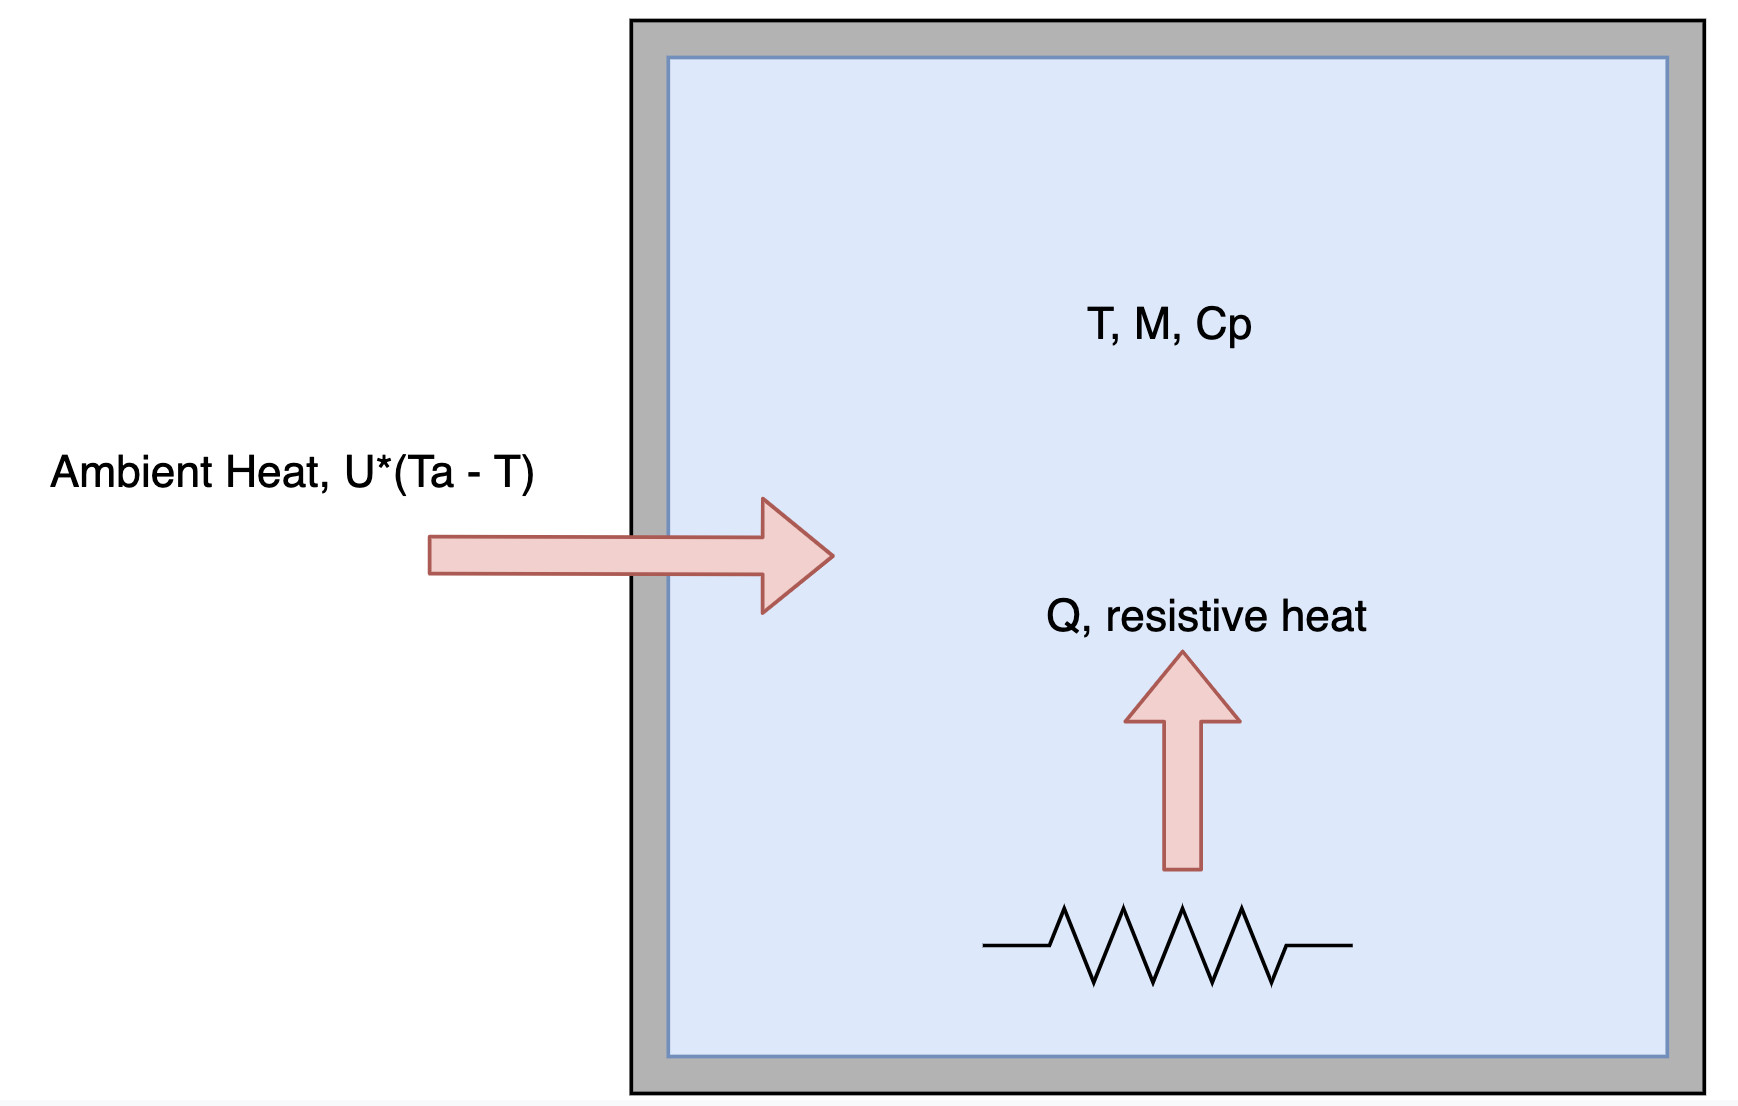
\includegraphics[scale=0.4]{plant}
  \caption{Plant}
\end{figure}

\subsubsection *{Modeling the System}

Thought process:
\begin{enumerate}
  \item The water forms one thermal inertia.
  \item Does the insulation have large enough an inertia to consider it as a second inertia or can I consider this as a purely conductive element? To ascertain this, I calculated the inertia of water and of the polyurethane \href{https://bit.ly/treaucalcs}{here} and found out a ratio of 30:1. So I modeled the polyurethane purely as a conductive element. 
\end{enumerate}

Math Model:
\\
\begin{equation}
\dot{T} = \frac{Q+U*(T_a-T)}{M*C_p}
\end{equation}
where: \\
T - Temperature of hot water tank \\
Q - controlled heat source \\
\(T_a\) - ambient temperature \\
M - mass of water \\
\(C_p\) - specific heat of water \\
\(U = \frac{k*A}{L} \) overall heat transfer coefficient of conduction
\newline
\newline
Rearranging: \\
\begin{equation}
M C_p \dot{T} + U T = Q + U T_a
\end{equation}

\noindent
\newline
This gives a transfer function of temperature over heat input as:
\begin{equation}
G(s) = \frac{T(s)}{Q(s)} = \frac{1}{M C_p s + U}
\end{equation}

%%%%%%%%%%%%%%%%%%%%
\subsection *{Designing the Controller}

Assume that the reference temperature (i.e. desired temperature) is \(T_{ref}\).
\noindent
\newline
\newline
Two considerations for the control design are:
\begin{enumerate}
  \item This is a first order linear system.
  \item This has a time delay.
\end{enumerate}
\noindent
For the first part:
\begin{enumerate}
  \item A feedforward component of \(U*(T_{ref} - T_a)\). I am adding this as there is a delay, so an open loop control will help in reaching the target.
  \item A feedback component \(C(s)\) - proportional control. In reality, a small integrator will also be required as the feedforward will not be perfect. The proportional gain can be tuned using stability/performance criteria.
\end{enumerate}
For the second part, I will augment the controller with a smith predictor. Here is how a smith predictor works:
\begin{enumerate}
  \item The process dynamics are \(G(s)*e^{-\tau s}\) where \(e^{-\tau s}\) is the laplace transform of the pure delay.
  \item The smith predictor can be understood in two steps:
  \begin{enumerate}
  \item Cancel out \(G(s)*e^{-\tau s}\)
  \item Replace it with the function \(G_p(s)\), which is a simulated version of \(G(s)\)
  \end{enumerate}
\end{enumerate}

\noindent
\newline
\newline
The process diagram with the controller is shown below. For reference, \textbf{blocks highlighted in \textcolor{TealBlue}{blue} are in in the ECU}, the rest is the real plant: \\

\begin{figure}[h!]
  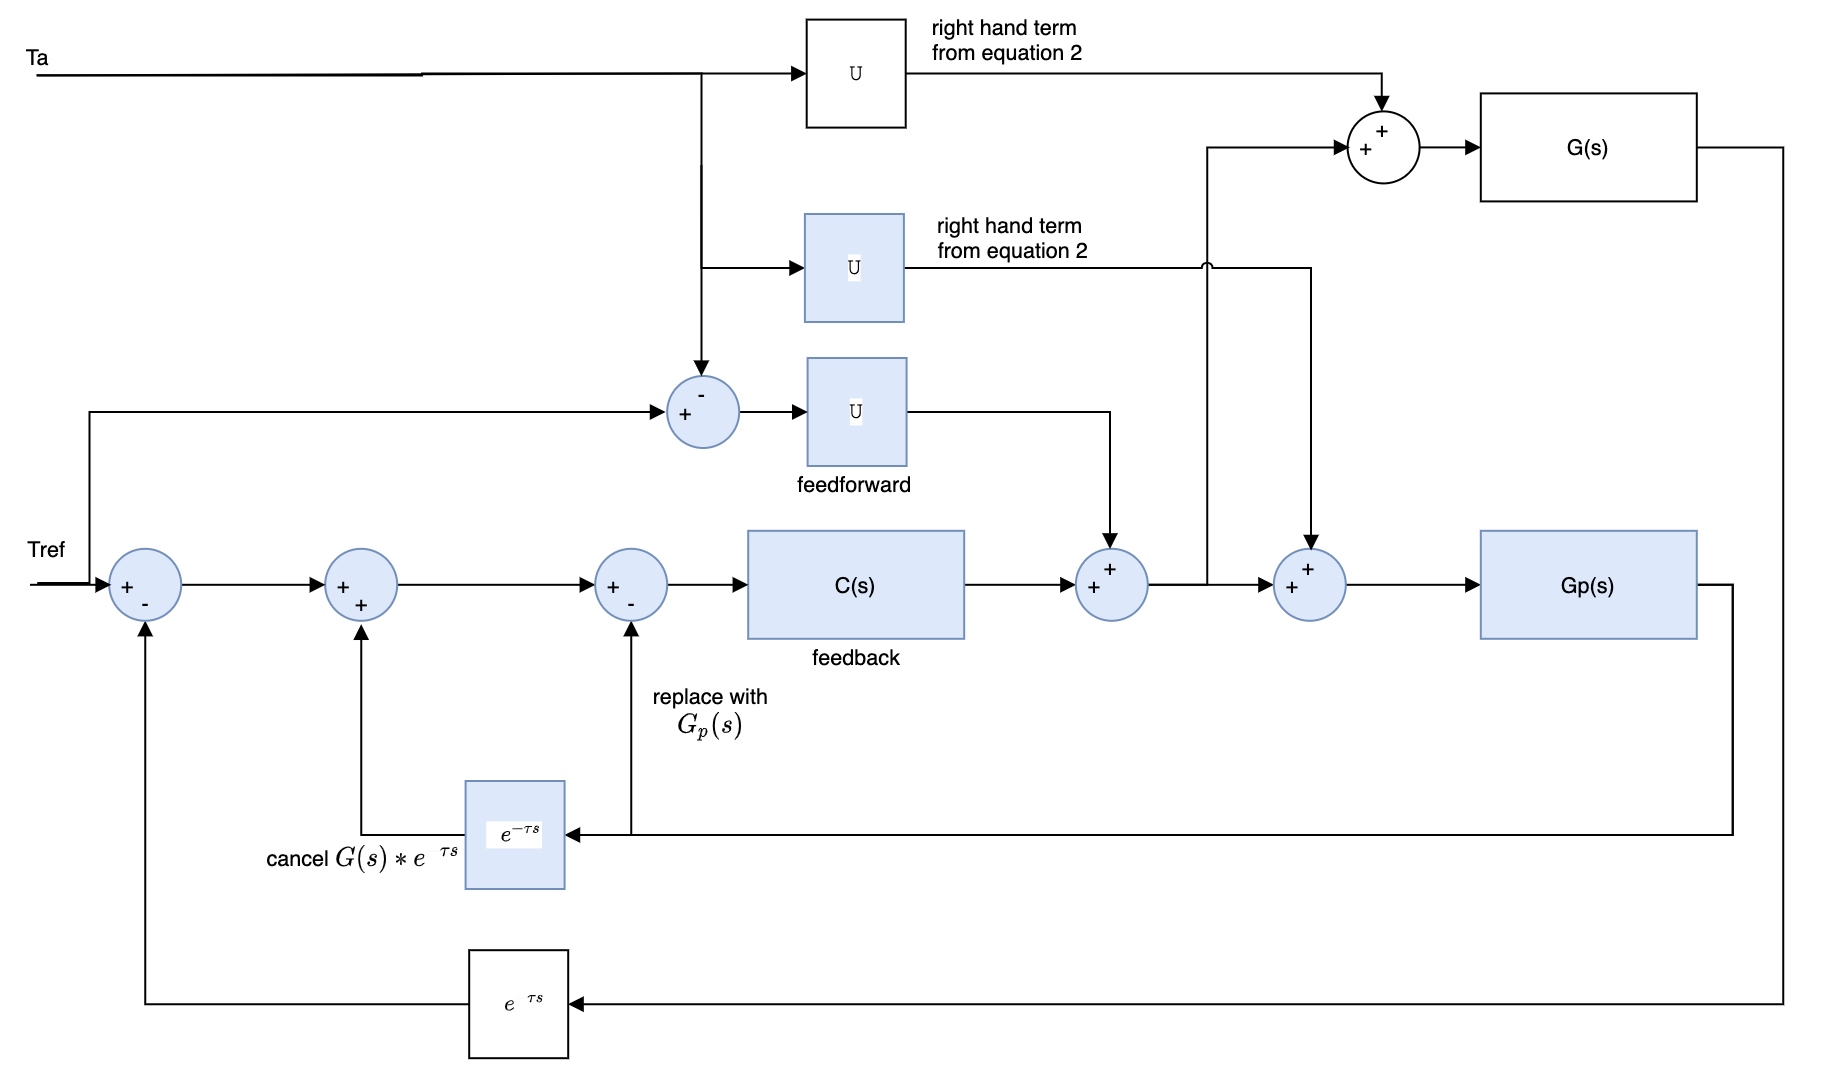
\includegraphics[width=\textwidth]{control_diagram}
  \caption{Process Diagram}
\end{figure}

%%%%%%%%%%%%%%
\subsection *{Parameters}
I used for polyurethane:
cp = 1800 J/kg-K
density = 132.953 Kg/$m^3$
conduction coefficient = 0.03 W/mK
\noindent
The closed loop transfer function with a proportional controller was:
\begin{equation}
G(s) = \frac{T(s)}{Q(s)} = \frac{K}{M C_p s + U + K} = \frac{K}{1.68 *10^7 s + 3.2 + K}
\end{equation}
\noindent
If I introduce a time constant requirement of 200 seconds, I get an extremely high gain of K = 82000. I googled residential hot water tanks and this gain would make the system be out of its actuating range for the most part.

%%%%%%%%%%%%%%
\subsection *{Hardware}
\begin{itemize}
  \item Thermistor - connected to ADC input with appropriately sized voltage divider circuit
  \item Resistive heater - not sure how this is throttled. If this was running off DC, I would use a half bridge that would have a PWM signal going to it from the micro.
  \item A micro of course for running the software.
  \item To input set temperature. Potentiometer to an ADC input.
  \item Display for temperature
\end{itemize}


\end{document}  